\section{Технический проект}
\subsection{Архитектура программной системы}

Разрабатываемая программная система представляет собой клиент-серверную web-платформу, предназначенную для поиска IT-вакансий и подбора IT-специалистов. Выбор клиент-серверной архитектуры обусловлен необходимостью разграничения пользовательского интерфейса, серверной логики и подсистемы хранения данных, а также поддержкой работы нескольких категорий пользователей в рамках единой программной среды. В системе предусмотрены роли неавторизованного пользователя, соискателя, работодателя и администратора, каждая из которых взаимодействует с платформой в пределах доступных ей функций.

Клиентская часть системы функционирует в браузере и предоставляет пользователю набор web-страниц для просмотра вакансий, регистрации и авторизации, ведения профиля соискателя, управления компанией работодателя, работы с откликами, избранными вакансиями и административными разделами. Доступ к пользовательскому интерфейсу осуществляется через набор маршрутов, соответствующих основным страницам платформы. Логика отображения данных и выполнения пользовательских действий реализуется на стороне клиента средствами HTML, CSS и JavaScript.

Серверная часть системы реализована в виде единого приложения на платформе Node.js с использованием фреймворка Express. Она построена по модульному принципу: маршруты (routes/), контроллеры (controllers/), сервисы (services/), промежуточные обработчики (middlewares/) и модели данных (models/) выделены в отдельные компоненты, что упрощает сопровождение и развитие системы. Сервер обрабатывает HTTP-запросы, выполняет маршрутизацию, проверяет права доступа через соответствующие middleware, реализует бизнес-логику и обеспечивает взаимодействие с базой данных. На уровне серверной логики можно выделить основные функциональные подсистемы: аутентификацию и управление пользователями, работу с профилем соискателя, управление навыками, ведение данных о компании, размещение и публикацию вакансий, обработку откликов, управление избранными вакансиями, поиск кандидатов и административное управление. Обмен данными между клиентской и серверной частями осуществляется через REST API, размещённый по префиксу /api.

Аутентификация пользователей построена на использовании JWT-токенов: при успешном входе клиент получает токен, который затем передаётся в заголовке Authorization при каждом защищённом запросе. Проверка токена и извлечение роли пользователя выполняются в middleware auth.middleware.js и role.middleware.js, что позволяет централизованно разграничивать доступ к функциям системы.

Подсистема хранения данных построена на основе реляционной системы управления базами данных PostgreSQL. Взаимодействие с ней осуществляется через ORM Sequelize, что обеспечивает объектно-ориентированный доступ к данным, параметризацию запросов и защиту от SQL-инъекций. База данных предназначена для хранения сведений о пользователях, профилях соискателей, компаниях, вакансиях, откликах, избранных вакансиях и навыках. Такое разделение позволяет обеспечить структурированное хранение информации, связность данных и поддержку основных процессов платформы, связанных с публикацией вакансий, поиском кандидатов и рассмотрением откликов.

С точки зрения организации взаимодействия компонентов работа системы осуществляется следующим образом. Пользователь через браузер открывает соответствующую страницу платформы и инициирует действие, например просмотр списка вакансий, отправку отклика, редактирование профиля или создание вакансии. Клиентская часть формирует запрос к серверу; серверное приложение принимает его, выполняет необходимую обработку (включая проверку прав, валидацию и обращение к сервисному слою), при необходимости взаимодействует с базой данных и возвращает результат клиенту в формате JSON. После этого интерфейс обновляется с учётом полученного ответа. Такой подход обеспечивает централизованную обработку данных, упрощает сопровождение системы и позволяет разграничить ответственность между уровнями представления, прикладной логики и хранения данных.

Дополнительно архитектура системы предусматривает возможность контейнеризированного развёртывания. В составе окружения используются контейнер приложения и контейнер базы данных, взаимодействующие между собой в рамках конфигурации Docker Compose. Это упрощает запуск системы, изоляцию компонентов и воспроизводимость программной среды при разработке и тестировании. Общая схема архитектуры программной системы представлена на рисунке 3.1.

\begin{figure}[H]
	\centering
	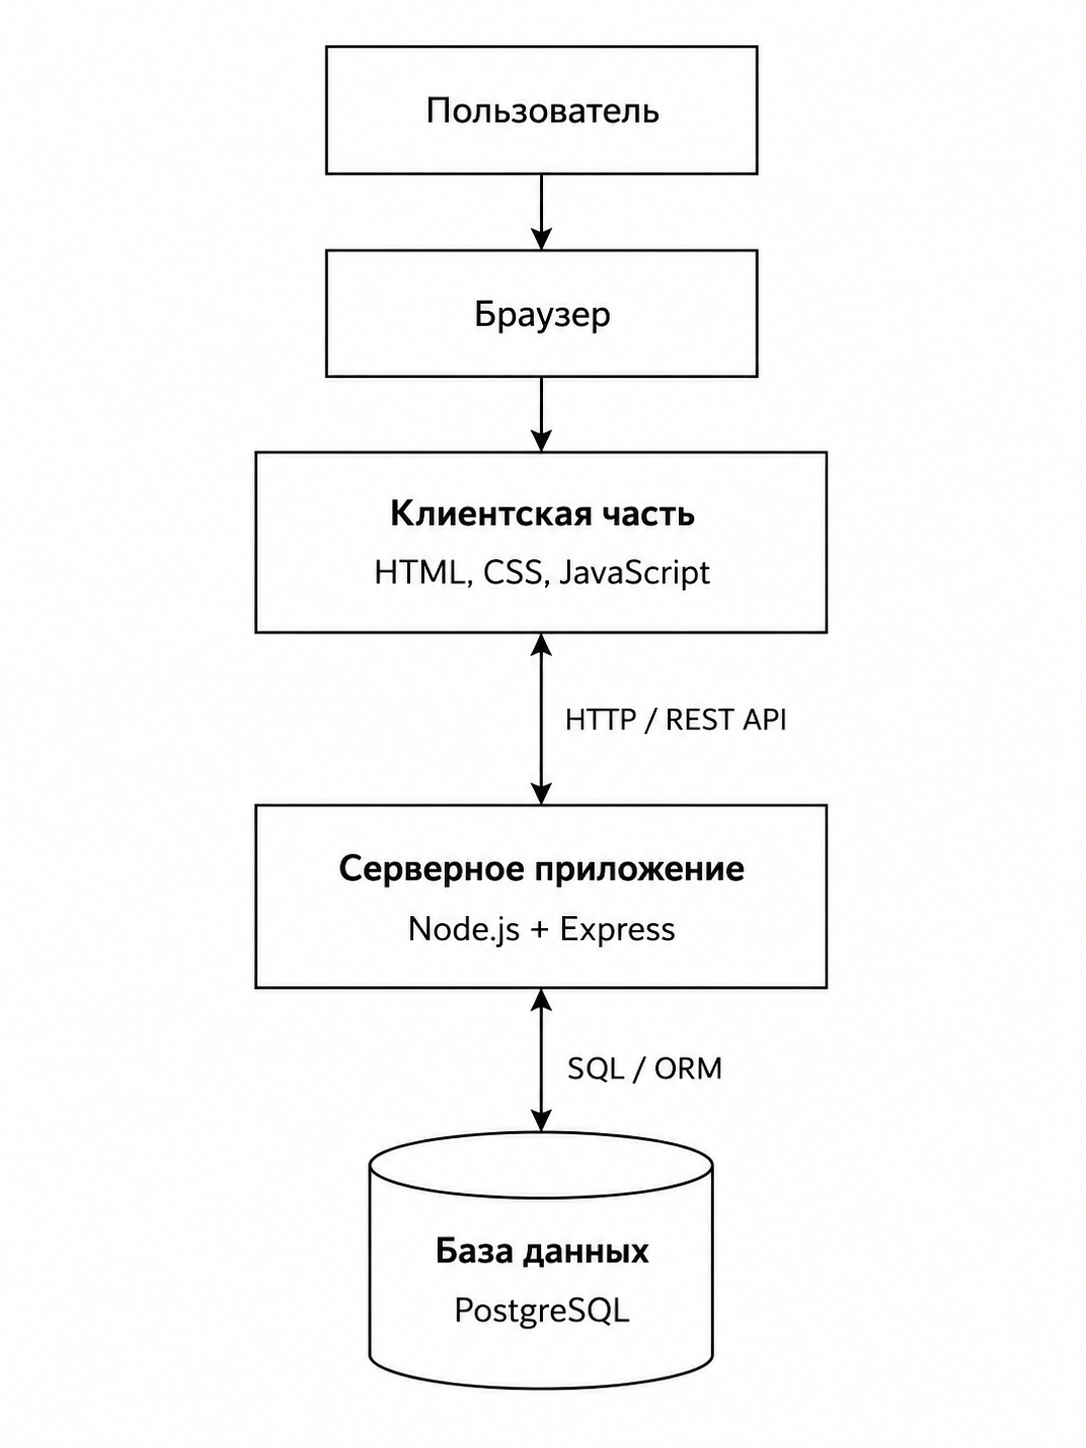
\includegraphics[width=0.70\linewidth]{fig_3_1_architecture.png}
	\caption{Архитектура программной системы}
	\label{fig:architecture}
\end{figure}

\subsection{Обоснование выбора технологий проектирования}

Выбор технологического стека для реализации платформы определялся архитектурой клиент-серверного web-приложения, необходимостью обеспечить надёжную обработку запросов, структурированное хранение данных, разграничение доступа пользователей и воспроизводимость программного окружения. В проекте используется стек, включающий Node.js, Express, PostgreSQL, Sequelize, JWT, bcryptjs, клиентские технологии HTML, CSS и JavaScript, а также Docker для контейнеризации среды выполнения.

В качестве серверной платформы выбрана Node.js. Это решение позволяет использовать JavaScript как на серверной, так и на клиентской стороне, что делает проект более однородным с точки зрения разработки и сопровождения. Для платформы это удобно, поскольку серверная часть реализует REST API, а клиентская часть построена на статических HTML-страницах с JavaScript-логикой, взаимодействующей с сервером через HTTP-запросы. Развитая экосистема npm также дала возможность применить необходимые библиотеки для маршрутизации, работы с базой данных, аутентификации и обработки cookie.

Веб-фреймворк Express использован для построения серверной части приложения. Он позволил организовать обработку HTTP-запросов, подключение middleware, раздачу статических файлов и маршрутизацию API по префиксу /api. В рамках проекта Express выступает основой единого серверного приложения, обслуживающего как клиентские страницы, так и программный интерфейс взаимодействия с данными платформы.

Для хранения данных выбрана система управления базами данных PostgreSQL. Данное решение подходит для платформы, в которой используются строго структурированные сущности и связи между ними: пользователи, профили соискателей, компании, вакансии, отклики, навыки и избранные вакансии. Применение реляционной СУБД позволяет обеспечить целостность данных, поддержку ограничений и надёжное хранение информации, задействованной в основных бизнес-процессах системы. Кроме того, PostgreSQL включена в состав контейнеризированного окружения проекта и запускается как отдельный сервис базы данных.

Для взаимодействия серверной части с базой данных применяется ORM Sequelize. Его использование позволило описывать модели и связи между ними на уровне приложения, управлять схемой базы данных через миграции и сократить объём рутинного кода при выполнении типовых операций чтения и записи. Для данного проекта это особенно важно из-за наличия нескольких связанных сущностей и промежуточных таблиц, обеспечивающих работу с навыками, откликами и избранными вакансиями.

Аутентификация пользователей реализована на основе механизма JWT. После успешного входа в систему сервер формирует токен, содержащий идентификатор пользователя, адрес электронной почты и его роль, после чего сохраняет этот токен в cookie. Дальнейшая проверка подлинности пользователя выполняется middleware серверной части, которое извлекает токен из cookie, проверяет его корректность и загружает сведения о текущем пользователе. Такой подход позволяет централизовать контроль доступа к защищённым маршрутам системы.

Для защиты паролей применяется библиотека bcryptjs. Перед сохранением в базе данных пароль преобразуется в хеш, что исключает хранение пользовательских паролей в открытом виде и повышает безопасность системы при работе с учётными записями.

Клиентская часть проекта реализована средствами HTML, CSS и JavaScript без использования дополнительных frontend-фреймворков. Такое решение соответствует структуре системы, в которой пользовательский интерфейс построен как набор отдельных страниц, каждая из которых отвечает за конкретный сценарий работы: просмотр вакансий, авторизацию, редактирование профиля, работу с откликами, управление вакансиями и административные действия. Отказ от отдельного frontend-фреймворка и этапа сборки упростил структуру проекта и сохранил достаточность клиентских средств для всех реализованных функций.

Для обеспечения единообразия программного окружения в проекте используется контейнеризация Docker. Конфигурация среды включает два основных сервиса: контейнер приложения и контейнер базы данных. Такой подход упрощает запуск системы, обеспечивает воспроизводимость окружения и изолирует основные компоненты платформы друг от друга.

Таким образом, выбранный технологический стек соответствует архитектуре разработанной платформы и обеспечивает реализацию серверной логики, клиентского интерфейса, хранения данных, аутентификации пользователей и контейнеризированного развёртывания системы.

\subsection{Клиентская часть}

Клиентская часть платформы представляет собой набор web-страниц, таблиц стилей CSS и клиентских JavaScript-скриптов, исполняемых в браузере пользователя. Серверная часть обеспечивает выдачу страниц и обработку API-запросов, а клиентская часть отвечает за отображение данных, обработку действий пользователя и динамическое обновление содержимого страниц.

Структура клиентской части организована в соответствии с основными пользовательскими ролями, предусмотренными в системе. Для неавторизованного пользователя доступны главная страница, страницы входа и регистрации, список опубликованных вакансий и карточка отдельной вакансии. На этих страницах реализованы просмотр опубликованных предложений, переход к подробной информации о вакансии и фильтрация вакансий по основным параметрам.

Интерфейс соискателя включает страницы ведения профиля, управления навыками, просмотра вакансий, отправки откликов, работы с избранными вакансиями и просмотра статусов ранее отправленных откликов. Через эти страницы соискатель может редактировать сведения о себе, управлять набором навыков, открывать карточки вакансий, отправлять отклики и отслеживать результаты взаимодействия с работодателями.

Интерфейс работодателя включает страницы управления данными компании, создания и редактирования вакансий, просмотра списка собственных вакансий, обработки откликов и поиска кандидатов. С помощью соответствующих форм работодатель может изменять сведения о компании, публиковать вакансии, снимать их с публикации, просматривать отклики, изменять их статус и выполнять поиск профилей соискателей по доступным параметрам.

Для администратора реализован отдельный интерфейс, предназначенный для просмотра пользователей и вакансий, а также выполнения административных действий. Через административные страницы обеспечиваются блокировка пользователей, снятие вакансий с публикации и удаление вакансий в пределах полномочий данной роли.

HTML-разметка страниц определяет структуру пользовательского интерфейса, включая формы ввода, списки объектов, карточки вакансий, элементы навигации и служебные блоки. Единое визуальное оформление страниц обеспечивается таблицами стилей CSS, размещёнными в каталоге public/css/. Использование общего набора стилей позволяет поддерживать единообразный внешний вид форм, карточек, списков и элементов управления во всех разделах платформы.

Динамическое поведение клиентской части реализуется с помощью JavaScript-скриптов, размещённых в каталоге public/js/. Они используются для загрузки данных с сервера через REST API, отправки данных форм, обработки ответов в формате JSON и изменения содержимого страниц в зависимости от результатов выполнения запроса. Такой подход позволяет отделить отображение данных в браузере от серверной бизнес-логики и обеспечить гибкое взаимодействие между пользовательским интерфейсом и серверной частью системы.

Обмен данными между клиентской и серверной частями осуществляется по модели «запрос–ответ». При выполнении пользовательского действия — открытии списка вакансий, сохранении профиля, создании вакансии или отправке отклика — клиентский скрипт формирует HTTP-запрос к соответствующему API-маршруту. Сервер обрабатывает запрос, выполняет необходимые операции и возвращает ответ, после чего интерфейс страницы обновляется в соответствии с полученными данными. Такой механизм позволяет реализовать интерактивное поведение страниц при сохранении общей простоты архитектуры клиентской части.

На стороне клиента также выполняется базовая проверка корректности вводимых данных перед их отправкой на сервер. При возникновении ошибки интерфейс отображает пользователю сообщение о невозможности выполнения операции, не раскрывая внутренние детали серверной реализации. Это повышает удобство работы с платформой и делает взаимодействие с системой более понятным для пользователя.

Таким образом, клиентская часть платформы обеспечивает реализацию всех пользовательских сценариев, связанных с просмотром вакансий, работой с профилем соискателя, управлением компанией и вакансиями, обработкой откликов и выполнением административных действий. Её структура соответствует ролевой модели системы и обеспечивает взаимодействие с серверной частью через REST API. Структура клиентской части и её взаимодействие с сервером представлены на рисунке 3.2.

\begin{figure}[H]
	\centering
	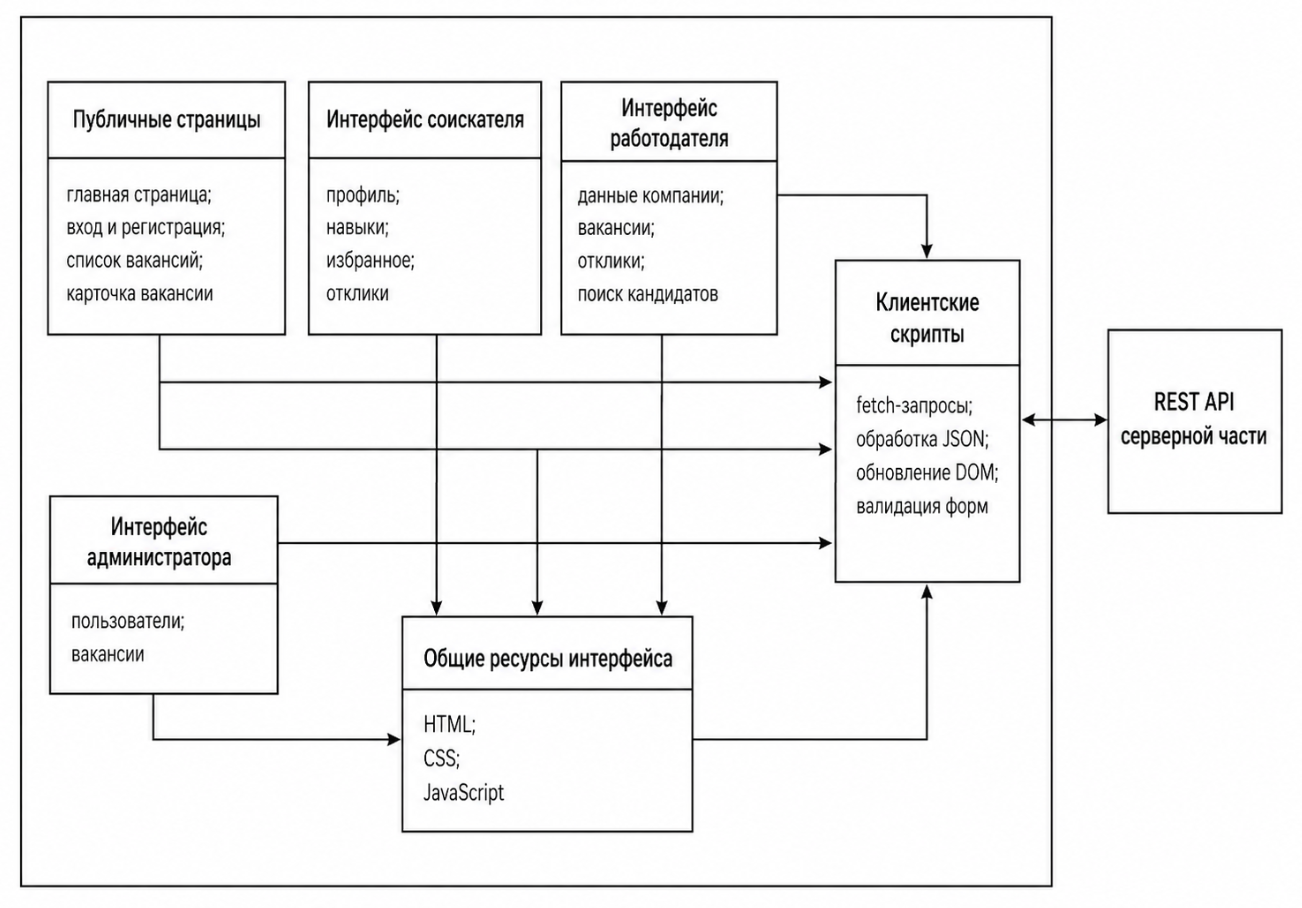
\includegraphics[width=0.79\linewidth]{fig_3_2_client_part.png}
	\caption{Структура клиентской части и её взаимодействие с сервером}
	\label{fig:client_part}
\end{figure}

\subsection{Серверная часть}

Серверная часть платформы построена по модульному принципу и включает маршруты API, промежуточные обработчики, контроллеры, сервисный слой и модели данных, взаимодействующие с базой данных PostgreSQL через ORM Sequelize. Структура серверной части представлена на рисунке 3.3.

\begin{figure}[H]
	\centering
	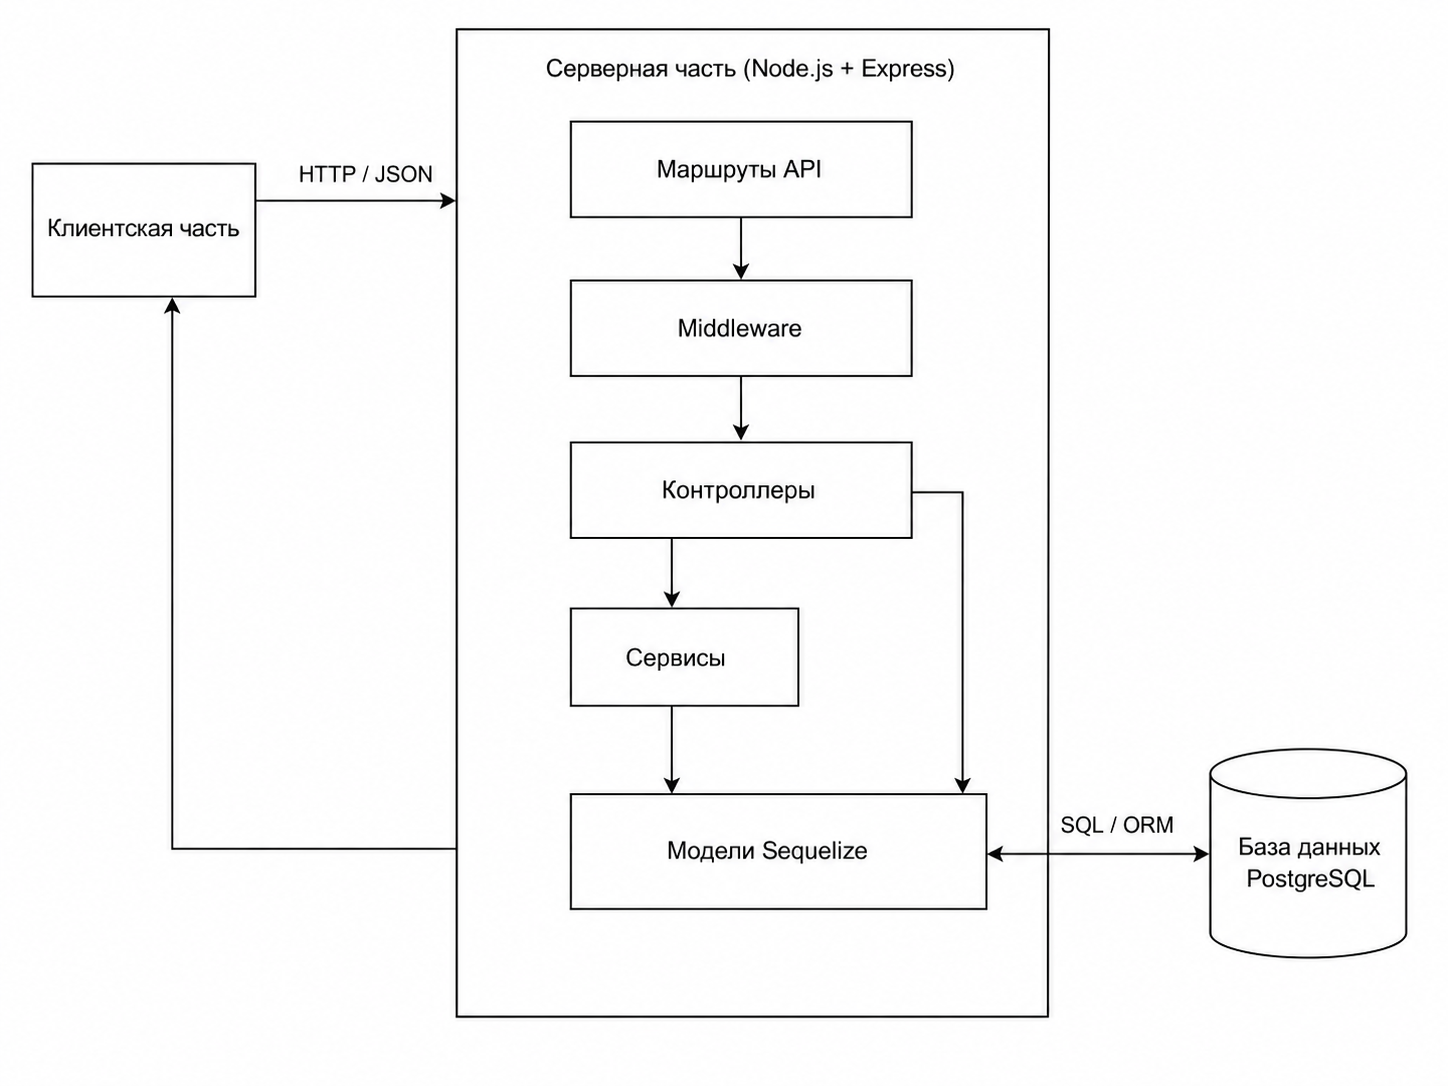
\includegraphics[width=\linewidth]{fig_3_3_server_part.png}
	\caption{Структура серверной части}
	\label{fig:server_part}
\end{figure}

Серверное приложение предоставляет REST API, через которое клиентская часть получает доступ к данным и выполняет основные операции программной системы. Маршруты API сгруппированы по функциональным подсистемам: аутентификация, работа с профилем соискателя, компанией, вакансиями, откликами, избранными вакансиями, навыками, пользовательскими и административными данными, а также приложения. Обмен данными между клиентской и серверной частями осуществляется в формате JSON. Доступ к части маршрутов открыт всем пользователям, тогда как операции, связанные с изменением данных и доступом к защищённым разделам системы, требуют аутентификации и, при необходимости, проверки роли пользователя. Далее приведено полное описание основных API-маршрутов программной системы с указанием их назначения, входных данных, структуры успешных JSON-ответов и основных ошибочных ситуаций.

\subsubsection{Служебный маршрут проверки работоспособности}

\textbf{Маршрут GET /api/health.}

Данный маршрут предназначен для проверки доступности серверного API. Он не требует аутентификации и может использоваться для контроля работоспособности серверной части приложения.

Path-параметры, query-параметры и тело запроса для данного маршрута отсутствуют.

При успешной обработке сервер возвращает ответ со статусом 200.

Пример успешного JSON-ответа:

\begin{flushleft}
	\small\ttfamily
	\{ "message": "API is working" \}
\end{flushleft}

Специальные бизнес-ошибки для данного маршрута не предусмотрены.

\subsubsection{Аутентификация}

Группа маршрутов аутентификации обеспечивает регистрацию пользователя, вход в систему, получение данных о текущем пользователе и завершение сессии. Основными маршрутами данной группы являются POST /api/auth/register, POST /api/auth/login, GET /api/auth/me и POST /api/auth/logout.

\textbf{Маршрут POST /api/auth/register.}

Маршрут предназначен для регистрации нового пользователя. Он доступен без предварительной аутентификации.

В теле запроса передаются поля email, password, fullName и role. Поле role может принимать только значения candidate или employer. Path-параметры и query-параметры отсутствуют.

При успешной регистрации сервер возвращает ответ со статусом 201 и JSON-объект, содержащий сообщение и краткие данные созданного пользователя.

Пример успешного JSON-ответа:

\begin{flushleft}
	\small\ttfamily
	\{ "message": "User registered successfully",\\
	"user": \{ "id": 1, "email": "candidate@example.com",\\
	"fullName": "Иван Иванов", "role": "candidate",\\
	"isBlocked": false \} \}
\end{flushleft}

Основные ошибки данного маршрута: 400 при отсутствии обязательных полей, недопустимой роли или попытке зарегистрировать уже существующий адрес электронной почты.

\textbf{Маршрут POST /api/auth/login.}

Маршрут предназначен для входа пользователя в систему. Он доступен без предварительной аутентификации.

В теле запроса передаются поля email и password. Path-параметры и query-параметры отсутствуют.

При успешной проверке учётных данных сервер возвращает ответ со статусом 200, формирует cookie token с JWT и передаёт JSON-объект с сообщением и краткими сведениями о пользователе.

Пример успешного JSON-ответа:

\begin{flushleft}
	\small\ttfamily
	\{ "message": "Login successful",\\
	"user": \{ "id": 1, "email": "candidate@example.com",\\
	"fullName": "Иван Иванов", "role": "candidate",\\
	"isBlocked": false \} \}
\end{flushleft}

Основные ошибки данного маршрута: 400 при отсутствии email или password, 401 при неверных учётных данных, 403 при попытке входа заблокированного пользователя.

\textbf{Маршрут GET /api/auth/me.}

Маршрут предназначен для получения сведений о текущем авторизованном пользователе. Доступ к нему имеет только пользователь с действительной сессией.

Входные данные в path, query и body отсутствуют, поскольку сведения о пользователе определяются на основе JWT-токена из cookie.

При успешной обработке сервер возвращает ответ со статусом 200 и JSON-объект с данными текущего пользователя.

Пример успешного JSON-ответа:

\begin{flushleft}
	\small\ttfamily
	\{ "message": "Current user",\\
	"user": \{ "id": 1, "email": "candidate@example.com",\\
	"fullName": "Иван Иванов", "role": "candidate",\\
	"isBlocked": false \} \}
\end{flushleft}

Основные ошибки данного маршрута: 401 при отсутствии или недействительности токена, 403 при блокировке пользователя.

\textbf{Маршрут POST /api/auth/logout.}

Маршрут предназначен для завершения пользовательской сессии. Он используется для удаления cookie token и завершения работы пользователя с системой.

Path-параметры, query-параметры и тело запроса отсутствуют.

При успешной обработке сервер возвращает ответ со статусом 200.

Пример успешного JSON-ответа:

\begin{flushleft}
	\small\ttfamily
	\{ "message": "Logout successful" \}
\end{flushleft}

Специальные бизнес-ошибки для данного маршрута не предусмотрены.

\subsubsection{Профиль соискателя}

Группа маршрутов профиля соискателя обеспечивает создание и редактирование профиля, просмотр собственного профиля, поиск и просмотр профилей работодателем, а также управление навыками профиля. Основными маршрутами данной группы являются GET /api/candidate-profile/me, POST /api/candidate-profile, PUT /api/candidate-profile/:id, GET /api/candidate-profile, GET /api/candidate-profile/:id, POST /api/candidate-profile/me/skills и DELETE /api/candidate-profile/me/skills/:skillId.

\textbf{Маршрут GET /api/candidate-profile/me.}

Маршрут предназначен для получения собственного профиля соискателя. Доступ к нему имеет только авторизованный пользователь с ролью candidate.

Path-параметры, query-параметры и тело запроса отсутствуют.

При успешной обработке сервер возвращает ответ со статусом 200 и JSON-объект с данными профиля и связанными навыками.

Пример успешного JSON-ответа:

\begin{flushleft}
	\small\ttfamily
	\{ "message": "Candidate profile fetched successfully",\\
	"profile": \{ "id": 1, "userId": 1,\\
	"specialization": "Backend-разработчик",\\
	"about": "Опыт работы с Node.js и PostgreSQL",\\
	"githubLink": "https://github.com/example",\\
	"skills": [\{ "id": 1, "name": "Node.js" \},\\
	\{ "id": 2, "name": "PostgreSQL" \}] \} \}
\end{flushleft}

Основные ошибки данного маршрута: 401 при отсутствии или недействительности токена, 403 при несоответствии роли, 404 при отсутствии профиля соискателя.

\textbf{Маршрут POST /api/candidate-profile.}

Маршрут предназначен для создания профиля соискателя. Доступ к нему имеет только авторизованный пользователь с ролью candidate.

В теле запроса передаются поля specialization, about и githubLink, где specialization является обязательным. Path-параметры и query-параметры отсутствуют.

При успешной обработке сервер возвращает ответ со статусом 201 и JSON-объект с данными созданного профиля.

Пример успешного JSON-ответа:

\begin{flushleft}
	\small\ttfamily
	\{ "message": "Candidate profile created successfully",\\
	"profile": \{ "id": 1, "userId": 1,\\
	"specialization": "Backend-разработчик",\\
	"about": "Опыт разработки серверных приложений",\\
	"githubLink": "https://github.com/example" \} \}
\end{flushleft}

Основные ошибки данного маршрута: 400 при отсутствии specialization или попытке создать профиль повторно, 401 при отсутствии аутентификации, 403 при несоответствии роли.

\textbf{Маршрут PUT /api/candidate-profile/:id.}

Маршрут предназначен для обновления ранее созданного профиля соискателя. Доступ к нему имеет только авторизованный пользователь с ролью candidate, причём изменять можно только собственный профиль.

Path-параметром является id профиля. В теле запроса могут передаваться поля specialization, about и githubLink. Query-параметры отсутствуют.

При успешной обработке сервер возвращает ответ со статусом 200 и JSON-объект с обновлёнными данными профиля.

Пример успешного JSON-ответа:

\begin{flushleft}
	\small\ttfamily
	\{ "message": "Candidate profile updated successfully",\\
	"profile": \{ "id": 1, "userId": 1,\\
	"specialization": "Backend-разработчик",\\
	"about": "Опыт Node.js, Express и PostgreSQL",\\
	"githubLink": "https://github.com/example" \} \}
\end{flushleft}

Основные ошибки данного маршрута: 400 при отсутствии полей для обновления, 403 при попытке изменять чужой профиль, 404 при отсутствии профиля.

\textbf{Маршрут GET /api/candidate-profile.}

Маршрут предназначен для получения списка профилей соискателей. Доступ к нему имеет только авторизованный пользователь с ролью employer.

Query-параметрами могут выступать specialization и skill, используемые для фильтрации результатов. Path-параметры и тело запроса отсутствуют.

При успешной обработке сервер возвращает ответ со статусом 200 и JSON-объект со списком профилей.

Пример успешного JSON-ответа:

\begin{flushleft}
	\small\ttfamily
	\{ "message": "Candidate profiles fetched successfully",\\
	"profiles": [\{ "id": 1,\\
	"specialization": "Backend-разработчик",\\
	"about": "Опыт Node.js",\\
	"githubLink": "https://github.com/example",\\
	"user": \{ "id": 1, "fullName": "Иван Иванов" \},\\
	"skills": [\{ "id": 1, "name": "Node.js" \}] \}] \}
\end{flushleft}

Основные ошибки данного маршрута: 401 при отсутствии аутентификации, 403 при несоответствии роли.

\textbf{Маршрут GET /api/candidate-profile/:id.}

Маршрут предназначен для просмотра конкретного профиля соискателя работодателем. Доступ к нему имеет только авторизованный пользователь с ролью employer.

Path-параметром является id профиля. Query-параметры и тело запроса отсутствуют.

При успешной обработке сервер возвращает ответ со статусом 200 и JSON-объект с данными выбранного профиля.

Пример успешного JSON-ответа:

\begin{flushleft}
	\small\ttfamily
	\{ "message": "Candidate profile fetched successfully",\\
	"profile": \{ "id": 1,\\
	"specialization": "Backend-разработчик",\\
	"about": "Опыт Node.js",\\
	"githubLink": "https://github.com/example",\\
	"user": \{ "id": 1, "fullName": "Иван Иванов" \},\\
	"skills": [\{ "id": 1, "name": "Node.js" \},\\
	\{ "id": 2, "name": "Express" \}] \} \}
\end{flushleft}

Основные ошибки данного маршрута: 401 при отсутствии аутентификации, 403 при несоответствии роли, 404 при отсутствии профиля.

\textbf{Маршрут POST /api/candidate-profile/me/skills.}

Маршрут предназначен для добавления навыка в собственный профиль соискателя. Доступ к нему имеет только авторизованный пользователь с ролью candidate.

В теле запроса передаётся поле name, содержащее название навыка. Path-параметры и query-параметры отсутствуют.

При успешной обработке сервер возвращает ответ со статусом 201 и JSON-объект с данными добавленного навыка.

Пример успешного JSON-ответа:

\begin{flushleft}
	\small\ttfamily
	\{ "message": "Skill added to candidate profile successfully",\\
	"skill": \{ "id": 3, "name": "Sequelize" \} \}
\end{flushleft}

Основные ошибки данного маршрута: 400 при отсутствии названия навыка или попытке добавить уже существующий навык, 404 при отсутствии профиля соискателя, 403 при несоответствии роли.

\textbf{Маршрут DELETE /api/candidate-profile/me/skills/:skillId.}

Маршрут предназначен для удаления навыка из собственного профиля соискателя. Доступ к нему имеет только авторизованный пользователь с ролью candidate.

Path-параметром является skillId. Query-параметры и тело запроса отсутствуют.

При успешной обработке сервер возвращает ответ со статусом 200.

Пример успешного JSON-ответа:

\begin{flushleft}
	\small\ttfamily
	\{ "message": "Skill removed from candidate profile successfully" \}
\end{flushleft}

Основные ошибки данного маршрута: 404 при отсутствии профиля или отсутствии указанного навыка в профиле, 403 при несоответствии роли.

\subsubsection{Компания работодателя}

Группа маршрутов компании предназначена для создания, просмотра и редактирования данных компании работодателя. Основными маршрутами данной группы являются GET /api/companies/my, POST /api/companies, PUT /api/companies/:id и GET /api/companies/:id.

\textbf{Маршрут GET /api/companies/my.}

Маршрут предназначен для получения собственной компании работодателя. Доступ к нему имеет только авторизованный пользователь с ролью employer.

Path-параметры, query-параметры и тело запроса отсутствуют.

При успешной обработке сервер возвращает ответ со статусом 200 и JSON-объект с данными компании.

Пример успешного JSON-ответа:

\begin{flushleft}
	\small\ttfamily
	\{ "message": "Company profile fetched successfully",\\
	"company": \{ "id": 1, "userId": 2,\\
	"name": "TechSoft",\\
	"description": "Разработка web-приложений",\\
	"website": "https://techsoft.example" \} \}
\end{flushleft}

Основные ошибки данного маршрута: 401 при отсутствии аутентификации, 403 при несоответствии роли, 404 при отсутствии профиля компании.

\textbf{Маршрут POST /api/companies.}

Маршрут предназначен для создания профиля компании работодателя. Доступ к нему имеет только авторизованный пользователь с ролью employer.

В теле запроса передаются поля name, description и website, где обязательным является поле name. Path-параметры и query-параметры отсутствуют.

При успешной обработке сервер возвращает ответ со статусом 201 и JSON-объект с данными созданной компании.

Пример успешного JSON-ответа:

\begin{flushleft}
	\small\ttfamily
	\{ "message": "Company profile created successfully",\\
	"company": \{ "id": 1, "userId": 2,\\
	"name": "TechSoft",\\
	"description": "Разработка серверных и клиентских приложений",\\
	"website": "https://techsoft.example" \} \}
\end{flushleft}

Основные ошибки данного маршрута: 400 при отсутствии name или попытке создать компанию повторно, 401 при отсутствии аутентификации, 403 при несоответствии роли.

\textbf{Маршрут PUT /api/companies/:id.}

Маршрут предназначен для обновления данных компании работодателя. Доступ к нему имеет только авторизованный пользователь с ролью employer, причём изменять можно только собственную компанию.

Path-параметром является id компании. В теле запроса могут передаваться поля name, description и website. Query-параметры отсутствуют.

При успешной обработке сервер возвращает ответ со статусом 200 и JSON-объект с обновлёнными данными компании.

Пример успешного JSON-ответа:

\begin{flushleft}
	\small\ttfamily
	\{ "message": "Company profile updated successfully",\\
	"company": \{ "id": 1, "userId": 2,\\
	"name": "TechSoft",\\
	"description": "Разработка web-систем для бизнеса",\\
	"website": "https://techsoft.example" \} \}
\end{flushleft}

Основные ошибки данного маршрута: 400 при отсутствии полей для обновления, 403 при попытке редактировать чужую компанию, 404 при отсутствии компании.

\textbf{Маршрут GET /api/companies/:id.}

Маршрут предназначен для получения данных конкретной компании работодателем. Доступ к нему имеет только авторизованный пользователь с ролью employer.

Path-параметром является id компании. Query-параметры и тело запроса отсутствуют.

При успешной обработке сервер возвращает ответ со статусом 200 и JSON-объект с данными компании.

Пример успешного JSON-ответа:

\begin{flushleft}
	\small\ttfamily
	\{ "message": "Company profile fetched successfully",\\
	"company": \{ "id": 1, "userId": 2,\\
	"name": "TechSoft",\\
	"description": "Разработка web-систем для бизнеса",\\
	"website": "https://techsoft.example" \} \}
\end{flushleft}

Основные ошибки данного маршрута: 401 при отсутствии аутентификации, 403 при несоответствии роли, 404 при отсутствии компании.

\subsubsection{Вакансии}

Группа маршрутов вакансий обеспечивает просмотр опубликованных вакансий, просмотр карточки отдельной вакансии, создание и редактирование вакансий работодателем, управление публикацией, работу с навыками вакансии, просмотр собственных вакансий, а также получение откликов по конкретной вакансии. Основными маршрутами данной группы являются GET /api/vacancies, GET /api/vacancies/:id, GET /api/vacancies/my, POST /api/vacancies, PUT /api/vacancies/:id, PATCH /api/vacancies/:id/publish, PATCH /api/vacancies/:id/unpublish, POST /api/vacancies/my/:id/skills, DELETE /api/vacancies/my/:id/skills/:skillId и GET /api/vacancies/:id/applications.

\textbf{Маршрут GET /api/vacancies.}

Маршрут предназначен для получения списка опубликованных вакансий. Доступ к нему открыт всем пользователям, включая неавторизованных.

В качестве query-параметров могут использоваться q или search для текстового поиска, specialization, workFormat или work\_format, employmentType или employment\_type, а также skill. Path-параметры и тело запроса отсутствуют.

При успешной обработке сервер возвращает ответ со статусом 200 и JSON-объект со списком вакансий.

Пример успешного JSON-ответа:

\begin{flushleft}
	\small\ttfamily
	\{ "message": "Vacancies fetched successfully",\\
	"vacancies": [\{ "id": 1, "title": "Backend Developer",\\
	"specialization": "Backend-разработчик",\\
	"description": "Разработка серверной части web-приложений",\\
	"requirements": "Node.js, PostgreSQL, REST API",\\
	"salary": "150000", "location": "Москва",\\
	"employmentType": "full\_time", "workFormat": "remote",\\
	"status": "published",\\
	"company": \{ "id": 1, "name": "TechSoft",\\
	"website": "https://techsoft.example" \},\\
	"skills": [\{ "id": 1, "name": "Node.js" \},\\
	\{ "id": 2, "name": "PostgreSQL" \}] \}] \}
\end{flushleft}

Специальные бизнес-ошибки для данного маршрута не предусмотрены.

\textbf{Маршрут GET /api/vacancies/:id.}

Маршрут предназначен для просмотра карточки конкретной опубликованной вакансии. Доступ к нему открыт всем пользователям, включая неавторизованных.

Path-параметром является id вакансии. Query-параметры и тело запроса отсутствуют.

При успешной обработке сервер возвращает ответ со статусом 200 и JSON-объект с данными выбранной вакансии.

Пример успешного JSON-ответа:

\begin{flushleft}
	\small\ttfamily
	\{ "message": "Vacancy fetched successfully",\\
	"vacancy": \{ "id": 1, "title": "Backend Developer",\\
	"specialization": "Backend-разработчик",\\
	"description": "Разработка серверной части web-приложений",\\
	"requirements": "Node.js, PostgreSQL, REST API",\\
	"salary": "150000", "location": "Москва",\\
	"employmentType": "full\_time", "workFormat": "remote",\\
	"status": "published",\\
	"company": \{ "id": 1, "name": "TechSoft",\\
	"description": "Разработка web-систем",\\
	"website": "https://techsoft.example" \},\\
	"skills": [\{ "id": 1, "name": "Node.js" \},\\
	\{ "id": 2, "name": "PostgreSQL" \}] \} \}
\end{flushleft}

Основные ошибки данного маршрута: 404 при отсутствии вакансии или невозможности её просмотра.

\textbf{Маршрут GET /api/vacancies/my.}

Маршрут предназначен для получения работодателем списка собственных вакансий. Доступ к нему имеет только авторизованный пользователь с ролью employer.

Path-параметры, query-параметры и тело запроса отсутствуют.

При успешной обработке сервер возвращает ответ со статусом 200 и JSON-объект со списком вакансий работодателя.

Пример успешного JSON-ответа:

\begin{flushleft}
	\small\ttfamily
	\{ "message": "Vacancies fetched successfully",\\
	"vacancies": [\{ "id": 1, "title": "Backend Developer",\\
	"specialization": "Backend-разработчик",\\
	"description": "Разработка серверной части web-приложений",\\
	"requirements": "Node.js, PostgreSQL",\\
	"salary": "150000", "location": "Москва",\\
	"employmentType": "full\_time", "workFormat": "remote",\\
	"status": "draft",\\
	"skills": [\{ "id": 1, "name": "Node.js" \},\\
	\{ "id": 2, "name": "PostgreSQL" \}] \}] \}
\end{flushleft}

Основные ошибки данного маршрута: 401 при отсутствии аутентификации, 403 при несоответствии роли, 404 при отсутствии профиля компании работодателя.

\textbf{Маршрут POST /api/vacancies.}

Маршрут предназначен для создания новой вакансии. Доступ к нему имеет только авторизованный пользователь с ролью employer.

В теле запроса передаются поля title, specialization, description, requirements, salary, location, employmentType, workFormat и status. Обязательными являются title, specialization, description, requirements, employmentType и workFormat. Path-параметры и query-параметры отсутствуют.

При успешной обработке сервер возвращает ответ со статусом 201 и JSON-объект с данными созданной вакансии.

Пример успешного JSON-ответа:

\begin{flushleft}
	\small\ttfamily
	\{ "message": "Vacancy created successfully",\\
	"vacancy": \{ "id": 1, "companyId": 1,\\
	"title": "Backend Developer",\\
	"specialization": "Backend-разработчик",\\
	"description": "Разработка серверной части web-приложений",\\
	"requirements": "Node.js, PostgreSQL",\\
	"salary": "150000", "location": "Москва",\\
	"employmentType": "full\_time", "workFormat": "remote",\\
	"status": "draft" \} \}
\end{flushleft}

Основные ошибки данного маршрута: 400 при отсутствии обязательных полей или недопустимых значениях employmentType, workFormat либо status, 401 при отсутствии аутентификации, 403 при несоответствии роли, 404 при отсутствии профиля компании работодателя.

\textbf{Маршрут PUT /api/vacancies/:id.}

Маршрут предназначен для обновления ранее созданной вакансии. Доступ к нему имеет только авторизованный пользователь с ролью employer, причём изменять можно только собственную вакансию.

Path-параметром является id вакансии. В теле запроса могут передаваться поля title, specialization, description, requirements, salary, location, employmentType, workFormat и status. Query-параметры отсутствуют.

При успешной обработке сервер возвращает ответ со статусом 200 и JSON-объект с обновлёнными данными вакансии.

Пример успешного JSON-ответа:

\begin{flushleft}
	\small\ttfamily
	\{ "message": "Vacancy updated successfully",\\
	"vacancy": \{ "id": 1, "companyId": 1,\\
	"title": "Backend Developer",\\
	"specialization": "Backend-разработчик",\\
	"description": "Разработка серверной части и API",\\
	"requirements": "Node.js, Express, PostgreSQL",\\
	"salary": "180000", "location": "Москва",\\
	"employmentType": "full\_time", "workFormat": "remote",\\
	"status": "draft" \} \}
\end{flushleft}

Основные ошибки данного маршрута: 400 при отсутствии полей для обновления или недопустимых значениях перечислимых полей, 401 при отсутствии аутентификации, 403 при несоответствии роли, 404 при отсутствии вакансии либо профиля компании.

\textbf{Маршрут PATCH /api/vacancies/:id/publish.}

Маршрут предназначен для публикации вакансии работодателем. Доступ к нему имеет только авторизованный пользователь с ролью employer.

Path-параметром является id вакансии. Query-параметры и тело запроса отсутствуют.

При успешной обработке сервер возвращает ответ со статусом 200 и JSON-объект с обновлённой вакансией.

Пример успешного JSON-ответа:

\begin{flushleft}
	\small\ttfamily
	\{ "message": "Vacancy published successfully",\\
	"vacancy": \{ "id": 1, "companyId": 1,\\
	"title": "Backend Developer",\\
	"specialization": "Backend-разработчик",\\
	"status": "published" \} \}
\end{flushleft}

Основные ошибки данного маршрута: 401 при отсутствии аутентификации, 403 при несоответствии роли, 404 при отсутствии вакансии или профиля компании.

\textbf{Маршрут PATCH /api/vacancies/:id/unpublish.}

Маршрут предназначен для снятия вакансии с публикации. Доступ к нему имеет авторизованный пользователь с ролью employer, а также администратор при выполнении модерационных действий.

Path-параметром является id вакансии. Query-параметры и тело запроса отсутствуют.

При успешной обработке сервер возвращает ответ со статусом 200 и JSON-объект с обновлённой вакансией.

Пример успешного JSON-ответа:

\begin{flushleft}
	\small\ttfamily
	\{ "message": "Vacancy unpublished successfully",\\
	"vacancy": \{ "id": 1, "companyId": 1,\\
	"title": "Backend Developer",\\
	"specialization": "Backend-разработчик",\\
	"status": "archived" \} \}
\end{flushleft}

Основные ошибки данного маршрута: 401 при отсутствии аутентификации, 403 при недостаточности прав доступа, 404 при отсутствии вакансии.

\textbf{Маршрут POST /api/vacancies/my/:id/skills.}

Маршрут предназначен для добавления навыка к вакансии работодателя. Доступ к нему имеет только авторизованный пользователь с ролью employer.

Path-параметром является id вакансии. В теле запроса передаётся поле name, содержащее название навыка. Query-параметры отсутствуют.

При успешной обработке сервер возвращает ответ со статусом 201 и JSON-объект с данными добавленного навыка.

Пример успешного JSON-ответа:

\begin{flushleft}
	\small\ttfamily
	\{ "message": "Skill added to vacancy successfully",\\
	"skill": \{ "id": 3, "name": "Sequelize" \} \}
\end{flushleft}

Основные ошибки данного маршрута: 400 при отсутствии названия навыка или попытке повторного добавления навыка, 401 при отсутствии аутентификации, 403 при несоответствии роли, 404 при отсутствии вакансии либо профиля компании.

\textbf{Маршрут DELETE /api/vacancies/my/:id/skills/:skillId.}

Маршрут предназначен для удаления навыка из вакансии работодателя. Доступ к нему имеет только авторизованный пользователь с ролью employer.

Path-параметрами являются id вакансии и skillId навыка. Query-параметры и тело запроса отсутствуют.

При успешной обработке сервер возвращает ответ со статусом 200.

Пример успешного JSON-ответа:

\begin{flushleft}
	\small\ttfamily
	\{ "message": "Skill removed from vacancy successfully" \}
\end{flushleft}

Основные ошибки данного маршрута: 401 при отсутствии аутентификации, 403 при несоответствии роли, 404 при отсутствии вакансии, профиля компании или указанного навыка в составе вакансии.

\textbf{Маршрут GET /api/vacancies/:id/applications.}

Маршрут предназначен для получения списка откликов на конкретную вакансию работодателя. Доступ к нему имеет только авторизованный пользователь с ролью employer.

Path-параметром является id вакансии. Query-параметры и тело запроса отсутствуют.

При успешной обработке сервер возвращает ответ со статусом 200 и JSON-объект со списком откликов.

Пример успешного JSON-ответа:

\begin{flushleft}
	\small\ttfamily
	\{ "message": "Applications fetched successfully",\\
	"applications": [\{ "id": 1, "status": "new",\\
	"candidateProfile": \{ "id": 1,\\
	"specialization": "Backend-разработчик",\\
	"about": "Опыт Node.js",\\
	"user": \{ "id": 1, "fullName": "Иван Иванов" \},\\
	"skills": [\{ "id": 1, "name": "Node.js" \}] \} \}] \}
\end{flushleft}

Основные ошибки данного маршрута: 401 при отсутствии аутентификации, 403 при несоответствии роли, 404 при отсутствии профиля компании либо вакансии работодателя.

\subsubsection{Отклики}

Группа маршрутов откликов предназначена для создания отклика на вакансию, просмотра собственных откликов соискателем и изменения статуса отклика работодателем. Основными маршрутами данной группы являются GET /api/applications/my, POST /api/applications и PATCH /api/applications/:id/status.

\textbf{Маршрут GET /api/applications/my.}

Маршрут предназначен для получения списка откликов текущего соискателя. Доступ к нему имеет только авторизованный пользователь с ролью candidate.

Path-параметры, query-параметры и тело запроса отсутствуют.

При успешной обработке сервер возвращает ответ со статусом 200 и JSON-объект со списком откликов.

Пример успешного JSON-ответа:

\begin{flushleft}
	\small\ttfamily
	\{ "message": "Applications fetched successfully",\\
	"applications": [\{ "id": 1, "status": "new",\\
	"vacancy": \{ "id": 3,\\
	"title": "Backend Developer",\\
	"specialization": "Backend-разработчик",\\
	"company": \{ "id": 1, "name": "TechSoft",\\
	"website": "https://techsoft.example" \} \} \}] \}
\end{flushleft}

Основные ошибки данного маршрута: 401 при отсутствии аутентификации, 403 при несоответствии роли, 404 при отсутствии профиля соискателя.

\textbf{Маршрут POST /api/applications.}

Маршрут предназначен для создания нового отклика на вакансию. Доступ к нему имеет только авторизованный пользователь с ролью candidate.

В теле запроса передаётся поле vacancyId. Path-параметры и query-параметры отсутствуют.

При успешной обработке сервер возвращает ответ со статусом 201 и JSON-объект с данными созданного отклика.

Пример успешного JSON-ответа:

\begin{flushleft}
	\small\ttfamily
	\{ "message": "Application created successfully",\\
	"application": \{ "id": 1, "vacancyId": 3,\\
	"profileId": 1, "status": "new" \} \}
\end{flushleft}

Основные ошибки данного маршрута: 400 при нечисловом vacancyId или повторной отправке отклика на ту же вакансию, 401 при отсутствии аутентификации, 403 при несоответствии роли, 404 при отсутствии профиля соискателя или опубликованной вакансии.

\textbf{Маршрут PATCH /api/applications/:id/status.}

Маршрут предназначен для изменения статуса отклика работодателем. Доступ к нему имеет только авторизованный пользователь с ролью employer.

Path-параметром является id отклика. В теле запроса передаётся поле status, которое может принимать значения new, in\_review, accepted или rejected. Query-параметры отсутствуют.

При успешной обработке сервер возвращает ответ со статусом 200 и JSON-объект с обновлённым откликом.

Пример успешного JSON-ответа:

\begin{flushleft}
	\small\ttfamily
	\{ "message": "Application status updated successfully",\\
	"application": \{ "id": 1, "vacancyId": 3,\\
	"profileId": 1, "status": "in\_review" \} \}
\end{flushleft}

Основные ошибки данного маршрута: 400 при недопустимом значении status, 401 при отсутствии аутентификации, 403 при несоответствии роли, 404 при отсутствии отклика или профиля компании работодателя.

\subsubsection{Избранные вакансии}

Группа маршрутов избранных вакансий обеспечивает добавление вакансии в избранное, удаление вакансии из избранного и просмотр списка сохранённых вакансий. Основными маршрутами данной группы являются GET /api/favorites, POST /api/favorites/:vacancyId и DELETE /api/favorites/:vacancyId.

\textbf{Маршрут GET /api/favorites.}

Маршрут предназначен для получения списка избранных вакансий текущего соискателя. Доступ к нему имеет только авторизованный пользователь с ролью candidate.

Path-параметры, query-параметры и тело запроса отсутствуют.

При успешной обработке сервер возвращает ответ со статусом 200 и JSON-объект со списком избранных вакансий.

Пример успешного JSON-ответа:

\begin{flushleft}
	\small\ttfamily
	\{ "message": "Favorite vacancies fetched successfully",\\
	"favorites": [\{ "id": 1,\\
	"vacancy": \{ "id": 3,\\
	"title": "Backend Developer",\\
	"specialization": "Backend-разработчик",\\
	"company": \{ "id": 1, "name": "TechSoft",\\
	"website": "https://techsoft.example" \} \} \}] \}
\end{flushleft}

Основные ошибки данного маршрута: 401 при отсутствии аутентификации, 403 при несоответствии роли.

\textbf{Маршрут POST /api/favorites/:vacancyId.}

Маршрут предназначен для добавления вакансии в список избранных. Доступ к нему имеет только авторизованный пользователь с ролью candidate.

Path-параметром является vacancyId. Query-параметры и тело запроса отсутствуют.

При успешной обработке сервер возвращает ответ со статусом 201 и JSON-объект с данными созданной записи избранного.

Пример успешного JSON-ответа:

\begin{flushleft}
	\small\ttfamily
	\{ "message": "Vacancy added to favorites successfully",\\
	"favorite": \{ "id": 1, "userId": 1,\\
	"vacancyId": 3 \} \}
\end{flushleft}

Основные ошибки данного маршрута: 400 при попытке повторно добавить ту же вакансию, 401 при отсутствии аутентификации, 403 при несоответствии роли, 404 при отсутствии опубликованной вакансии.

\textbf{Маршрут DELETE /api/favorites/:vacancyId.}

Маршрут предназначен для удаления вакансии из списка избранных. Доступ к нему имеет только авторизованный пользователь с ролью candidate.

Path-параметром является vacancyId. Query-параметры и тело запроса отсутствуют.

При успешной обработке сервер возвращает ответ со статусом 200.

Пример успешного JSON-ответа:

\begin{flushleft}
	\small\ttfamily
	\{ "message": "Vacancy removed from favorites successfully" \}
\end{flushleft}

Основные ошибки данного маршрута: 401 при отсутствии аутентификации, 403 при несоответствии роли, 404 при отсутствии вакансии в списке избранного.

\subsubsection{Навыки}

Группа маршрутов навыков представлена маршрутом GET /api/skills, который используется для получения справочного списка навыков, доступных в системе.

\textbf{Маршрут GET /api/skills.}

Маршрут предназначен для получения общего списка навыков. Доступ к нему имеет любой авторизованный пользователь независимо от роли.

Path-параметры, query-параметры и тело запроса отсутствуют.

При успешной обработке сервер возвращает ответ со статусом 200 и JSON-объект со списком навыков.

Пример успешного JSON-ответа:

\begin{flushleft}
	\small\ttfamily
	\{ "message": "Skills fetched successfully",\\
	"skills": [\{ "id": 1, "name": "Node.js" \},\\
	\{ "id": 2, "name": "PostgreSQL" \},\\
	\{ "id": 3, "name": "Express" \}] \}
\end{flushleft}

Основные ошибки данного маршрута: 401 при отсутствии аутентификации или недействительности сессии.

\subsubsection{Пользовательские маршруты}

Группа пользовательских маршрутов представлена маршрутами GET /api/users/:id и PUT /api/users/:id. Эти маршруты используются для получения и обновления данных собственной учётной записи пользователя.

\textbf{Маршрут GET /api/users/:id.}

Маршрут предназначен для получения данных пользователя по его идентификатору. Доступ к нему имеет только авторизованный пользователь, причём получить можно только данные собственной учётной записи.

Path-параметром является id пользователя. Query-параметры и тело запроса отсутствуют.

При успешной обработке сервер возвращает ответ со статусом 200 и JSON-объект с данными пользователя.

Пример успешного JSON-ответа:

\begin{flushleft}
	\small\ttfamily
	\{ "message": "User fetched successfully",\\
	"user": \{ "id": 1,\\
	"email": "candidate@example.com",\\
	"fullName": "Иван Иванов",\\
	"role": "candidate",\\
	"isBlocked": false \} \}
\end{flushleft}

Основные ошибки данного маршрута: 400 при некорректном формате id, 401 при отсутствии аутентификации, 403 при попытке получить данные другого пользователя, 404 при отсутствии пользователя.

\textbf{Маршрут PUT /api/users/:id.}

Маршрут предназначен для обновления данных собственной учётной записи пользователя. Доступ к нему имеет только авторизованный пользователь, причём изменять можно только собственные данные.

Path-параметром является id пользователя. В теле запроса могут передаваться поля email и fullName. Query-параметры отсутствуют.

При успешной обработке сервер возвращает ответ со статусом 200 и JSON-объект с обновлёнными данными пользователя.

Пример успешного JSON-ответа:

\begin{flushleft}
	\small\ttfamily
	\{ "message": "User updated successfully",\\
	"user": \{ "id": 1,\\
	"email": "candidate@example.com",\\
	"fullName": "Иван Иванов",\\
	"role": "candidate",\\
	"isBlocked": false \} \}
\end{flushleft}

Основные ошибки данного маршрута: 400 при отсутствии полей для обновления, пустом значении email или fullName, а также при попытке использовать уже занятый адрес электронной почты, 401 при отсутствии аутентификации, 403 при попытке изменить данные другого пользователя, 404 при отсутствии пользователя.

\subsubsection{Административные маршруты}

Группа административных маршрутов обеспечивает просмотр пользователей и вакансий, блокировку пользователя и удаление вакансии. Основными маршрутами данной группы являются GET /api/admin/users, GET /api/admin/vacancies, PATCH /api/admin/users/:id/block и DELETE /api/admin/vacancies/:id.

\textbf{Маршрут GET /api/admin/users.}

Маршрут предназначен для получения списка пользователей программной системы. Доступ к нему имеет только авторизованный пользователь с ролью admin.

Path-параметры, query-параметры и тело запроса отсутствуют.

При успешной обработке сервер возвращает ответ со статусом 200 и JSON-объект со списком пользователей.

Пример успешного JSON-ответа:

\begin{flushleft}
	\small\ttfamily
	\{ "message": "Users fetched successfully",\\
	"users": [\{ "id": 1,\\
	"email": "candidate@example.com",\\
	"fullName": "Иван Иванов",\\
	"role": "candidate",\\
	"isBlocked": false \},\\
	\{ "id": 2,\\
	"email": "employer@example.com",\\
	"fullName": "ООО ТехСофт",\\
	"role": "employer",\\
	"isBlocked": false \}] \}
\end{flushleft}

Основные ошибки данного маршрута: 401 при отсутствии аутентификации, 403 при несоответствии роли.

\textbf{Маршрут GET /api/admin/vacancies.}

Маршрут предназначен для получения списка вакансий программной системы администратором. Доступ к нему имеет только авторизованный пользователь с ролью admin.

Path-параметры, query-параметры и тело запроса отсутствуют.

При успешной обработке сервер возвращает ответ со статусом 200 и JSON-объект со списком вакансий.

Пример успешного JSON-ответа:

\begin{flushleft}
	\small\ttfamily
	\{ "message": "Vacancies fetched successfully",\\
	"vacancies": [\{ "id": 1,\\
	"title": "Backend Developer",\\
	"specialization": "Backend-разработчик",\\
	"status": "published",\\
	"company": \{ "id": 1, "name": "TechSoft",\\
	"website": "https://techsoft.example" \} \}] \}
\end{flushleft}

Основные ошибки данного маршрута: 401 при отсутствии аутентификации, 403 при несоответствии роли.

\textbf{Маршрут PATCH /api/admin/users/:id/block.}

Маршрут предназначен для блокировки пользователя администратором. Доступ к нему имеет только авторизованный пользователь с ролью admin.

Path-параметром является id пользователя. Query-параметры и тело запроса отсутствуют.

При успешной обработке сервер возвращает ответ со статусом 200 и JSON-объект с обновлёнными данными пользователя.

Пример успешного JSON-ответа:

\begin{flushleft}
	\small\ttfamily
	\{ "message": "User blocked successfully",\\
	"user": \{ "id": 1,\\
	"email": "candidate@example.com",\\
	"fullName": "Иван Иванов",\\
	"role": "candidate",\\
	"isBlocked": true \} \}
\end{flushleft}

Основные ошибки данного маршрута: 401 при отсутствии аутентификации, 403 при несоответствии роли, 404 при отсутствии пользователя, 400 при попытке администратора заблокировать собственную учётную запись.

\textbf{Маршрут DELETE /api/admin/vacancies/:id.}

Маршрут предназначен для удаления вакансии администратором. Доступ к нему имеет только авторизованный пользователь с ролью admin.

Path-параметром является id вакансии. Query-параметры и тело запроса отсутствуют.

При успешной обработке сервер возвращает ответ со статусом 200.

Пример успешного JSON-ответа:

\begin{flushleft}
	\small\ttfamily
	\{ "message": "Vacancy deleted successfully" \}
\end{flushleft}

Основные ошибки данного маршрута: 401 при отсутствии аутентификации, 403 при несоответствии роли, 404 при отсутствии вакансии.

В качестве иллюстрации взаимодействия компонентов серверной части рассмотрим процесс обработки запроса на создание отклика на вакансию. Данный сценарий реализуется через маршрут POST /api/applications и охватывает основные уровни серверной архитектуры: маршрутизацию, аутентификацию, проверку роли пользователя, работу контроллера, вызов сервисного слоя и обращение к базе данных. Такой пример является показательным для рассматриваемой платформы, поскольку объединяет несколько ключевых механизмов серверной обработки в рамках одного пользовательского действия.

Клиентская часть, работающая в браузере соискателя, отправляет POST-запрос на адрес /api/applications, передавая в теле запроса идентификатор вакансии vacancyId. При этом запрос включает cookie с JWT-токеном, который используется сервером для установления личности пользователя. После поступления запроса Express-маршрутизатор передаёт его в цепочку обработки, заданную для данного маршрута.

На первом этапе выполняется middleware аутентификации auth.middleware.js. Оно извлекает токен из req.cookies.token, проверяет его корректность, после чего загружает пользователя из базы данных. Если токен отсутствует, недействителен, срок его действия истёк, пользователь не найден или его учётная запись заблокирована, запрос завершается с ошибкой 401 или 403. При успешной проверке middleware формирует объект req.user, содержащий идентификатор пользователя, его адрес электронной почты, имя, роль и признак блокировки.

После успешной аутентификации выполняется role.middleware.js, которому для данного маршрута передаётся роль ROLES.CANDIDATE. Это middleware проверяет наличие объекта req.user и убеждается, что текущий пользователь является соискателем. Если роль не соответствует требуемой, сервер немедленно возвращает ответ с кодом 403 и сообщением о недостаточности прав доступа.

Если оба middleware завершились успешно, управление передаётся функции createApplication в application.controller.js. На уровне контроллера выполняется базовая проверка входных данных: значение vacancyId должно иметь числовой формат. При нарушении этого условия контроллер сразу возвращает ответ с кодом 400 и сообщением об ошибке. Если проверка проходит успешно, контроллер вызывает сервисный метод applicationService.createApplication(req.user.id, vacancyId).

Основная бизнес-логика создания отклика сосредоточена в application.service.js. Сначала сервис ищет профиль соискателя, связанный с текущим пользователем. Если профиль отсутствует, формируется ошибка 404. Затем сервис выполняет поиск вакансии по переданному идентификатору и одновременно проверяет, что её статус равен published. Если подходящая опубликованная вакансия не найдена, также возвращается ошибка 404. После этого выполняется проверка на наличие уже существующего отклика от данного соискателя на ту же вакансию. Если такой отклик уже есть, формируется ошибка 400. При успешном прохождении всех проверок сервис создаёт новую запись Application в базе данных со статусом new.

После создания отклика сервис возвращает контроллеру созданный объект. Контроллер, в свою очередь, формирует HTTP-ответ со статусом 201 и JSON-телом, содержащим сообщение об успешном создании отклика и данные созданной записи. Таким образом, на уровне клиента операция завершается получением подтверждения о выполнении действия и обновлением интерфейса в соответствии с результатом запроса.

Обработка ошибок в данном сценарии организована комбинированным образом. Часть ошибок возвращается непосредственно в middleware или контроллере, например при отсутствии прав доступа или неверном формате vacancyId. Ошибки, возникающие в сервисном слое или передаваемые через next(error), обрабатываются централизованным error.middleware.js, который возвращает JSON-ответ с полем message и соответствующим HTTP-статусом. Такой подход позволяет сохранить единый формат ответа об ошибке, при этом не все ошибочные ситуации проходят через единый обработчик.

Рассмотренный процесс демонстрирует последовательное взаимодействие основных элементов серверной части: маршрута, middleware аутентификации и проверки роли, контроллера, сервисного слоя и базы данных. Диаграмма последовательности, иллюстрирующая обработку запроса на создание отклика на вакансию, приведена на рисунке 3.4.

\clearpage
\begingroup
\setlength{\textwidth}{\paperwidth}
\begin{landscape}
	\thispagestyle{plain}
	\centering
	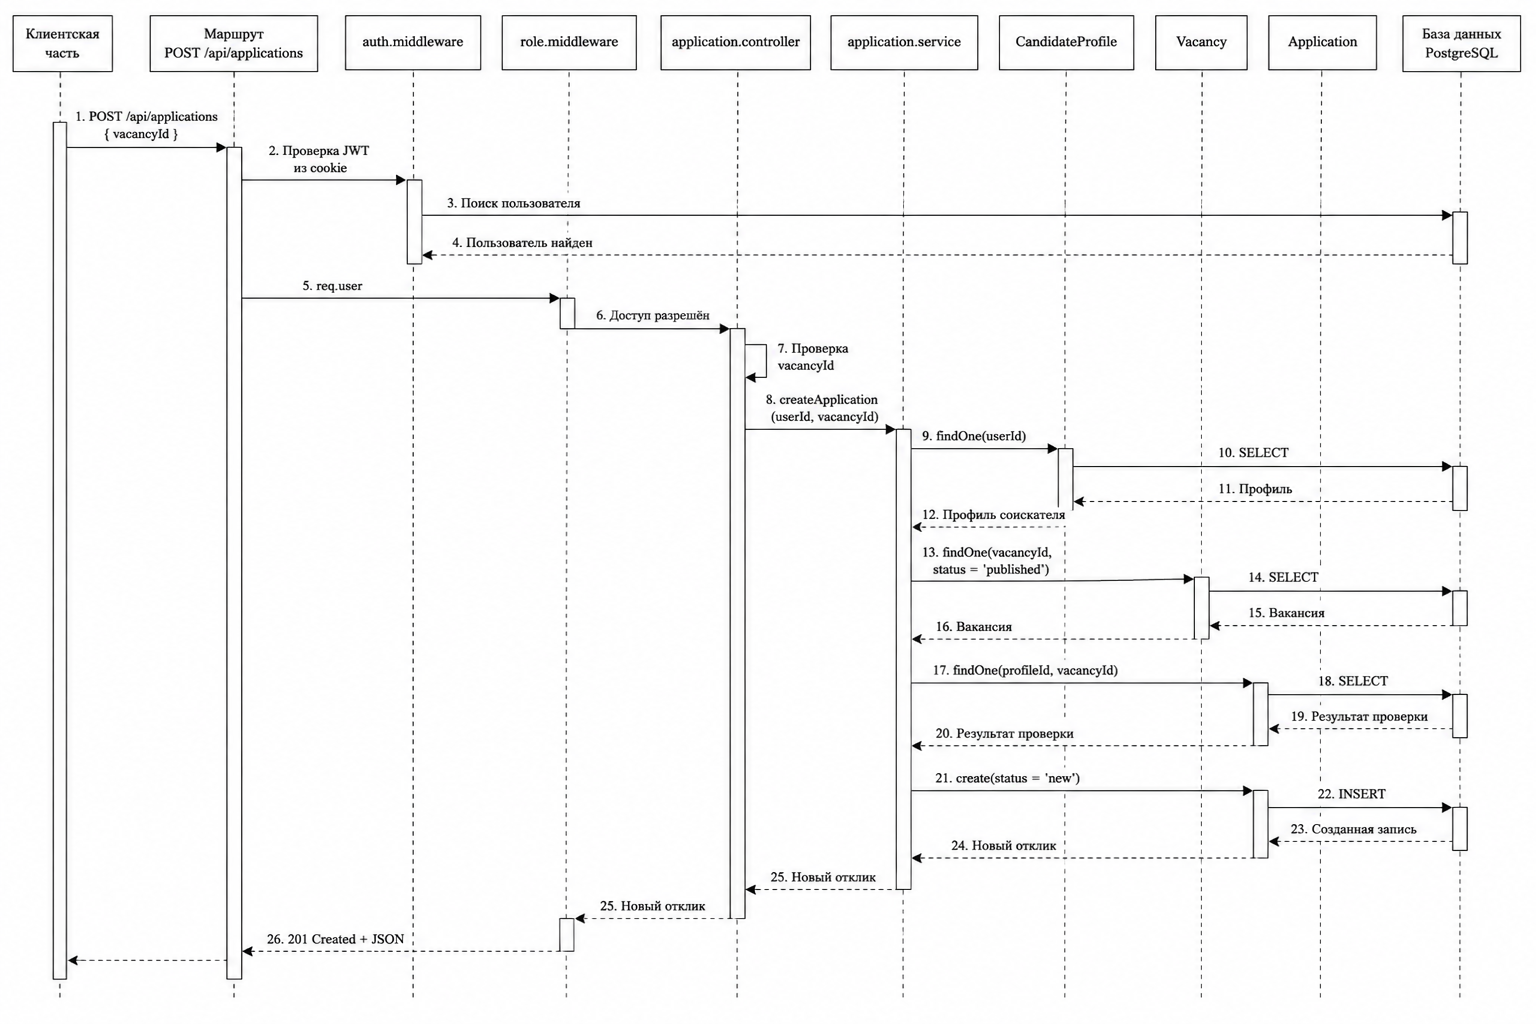
\includegraphics[width=\linewidth]{fig_3_4_request_sequence.png}
	
	\captionof{figure}{Диаграмма последовательности обработки запроса на создание отклика}
	\label{fig:request_sequence}
\end{landscape}
\endgroup

\subsection{Проект базы данных программно-информационной системы}

\subsubsection{ER-модель данных (включая основные сущности и связи)}

ER-модель данных разработанной платформы отражает логическую структуру предметной области и фиксирует основные сущности системы, их смысловые атрибуты и связи между ними. На концептуальном уровне модель описывает пользователей платформы, профессиональные сведения соискателей, данные работодателей, вакансии, навыки, отклики и избранные вакансии. Такая структура соответствует назначению системы, ориентированной на поиск работы и подбор IT-специалистов.

Центральной сущностью модели является пользователь (User), представляющий учётную запись в системе. Для пользователя хранятся адрес электронной почты, хеш пароля, полное имя, роль и признак блокировки. Роль пользователя задаётся значением атрибута и не выносится в самостоятельную сущность, что позволяет использовать единую модель учётной записи для соискателей, работодателей и администраторов.

Сущность CandidateProfile содержит профессиональные сведения соискателя. Она связана с сущностью User отношением «один к одному» на уровне модели предметной области: одному пользователю может соответствовать не более одного профиля соискателя. Профиль включает специализацию, краткое описание и ссылку на GitHub. Таким образом, профессиональные данные соискателя хранятся в отдельной сущности, связанной с его учётной записью.

Сущность Company представляет работодателя как организацию, публикующую вакансии на платформе. Она также связана с User отношением «один к одному»: одному пользователю может соответствовать не более одной компании. В составе сущности хранятся название компании, её описание и адрес веб-сайта. Такое разделение позволяет разграничить общие данные учётной записи и сведения, относящиеся непосредственно к работодателю.

Сущность Vacancy описывает предложение работы, размещаемое компанией. Каждая вакансия связана с одной компанией, при этом одна компания может размещать множество вакансий. В составе вакансии хранятся название, специализация, описание, требования, сведения о заработной плате, местоположение, тип занятости, формат работы, статус публикации и дата создания. Таким образом, между Company и Vacancy реализуется связь «один ко многим».

Сущность Skill используется как справочник навыков, применяемый в системе для описания требований вакансий и профессиональных характеристик соискателей. Связь между профилем соискателя и навыком реализуется через ассоциативную сущность CandidateSkill, что соответствует отношению «многие ко многим». Аналогично связь между вакансией и навыком реализуется через ассоциативную сущность VacancySkill, которая также отражает отношение «многие ко многим». Такое решение позволяет использовать единый перечень навыков для разных объектов предметной области.

Сущность Application фиксирует факт отклика соискателя на конкретную вакансию. Она связывает профиль соискателя и вакансию: один профиль может иметь множество откликов, и одна вакансия может получать множество откликов. В составе отклика хранятся ссылка на профиль, ссылка на вакансию, статус обработки и дата создания. Тем самым сущность Application отражает процесс взаимодействия между соискателем и работодателем в рамках конкретной вакансии.

Сущность FavoriteVacancy реализует связь между пользователем и вакансиями, добавленными в избранное. В данном случае избранное связано именно с учётной записью пользователя, а не с профилем соискателя. Это позволяет хранить перечень вакансий, отмеченных пользователем для последующего просмотра, в виде отдельной ассоциативной сущности, формирующей отношение «многие ко многим» между User и Vacancy.

В целом ER-модель образует целостную структуру, в которой учётная запись пользователя служит отправной точкой для ролевых сценариев работы с системой, компании размещают вакансии, соискатели ведут профессиональный профиль и откликаются на вакансии, а навыки используются как общий справочник для описания требований и компетенций. ER-диаграмма, отражающая указанные сущности и связи между ними, представлена на рисунке 3.5.

\begin{figure}[H]
	\centering
	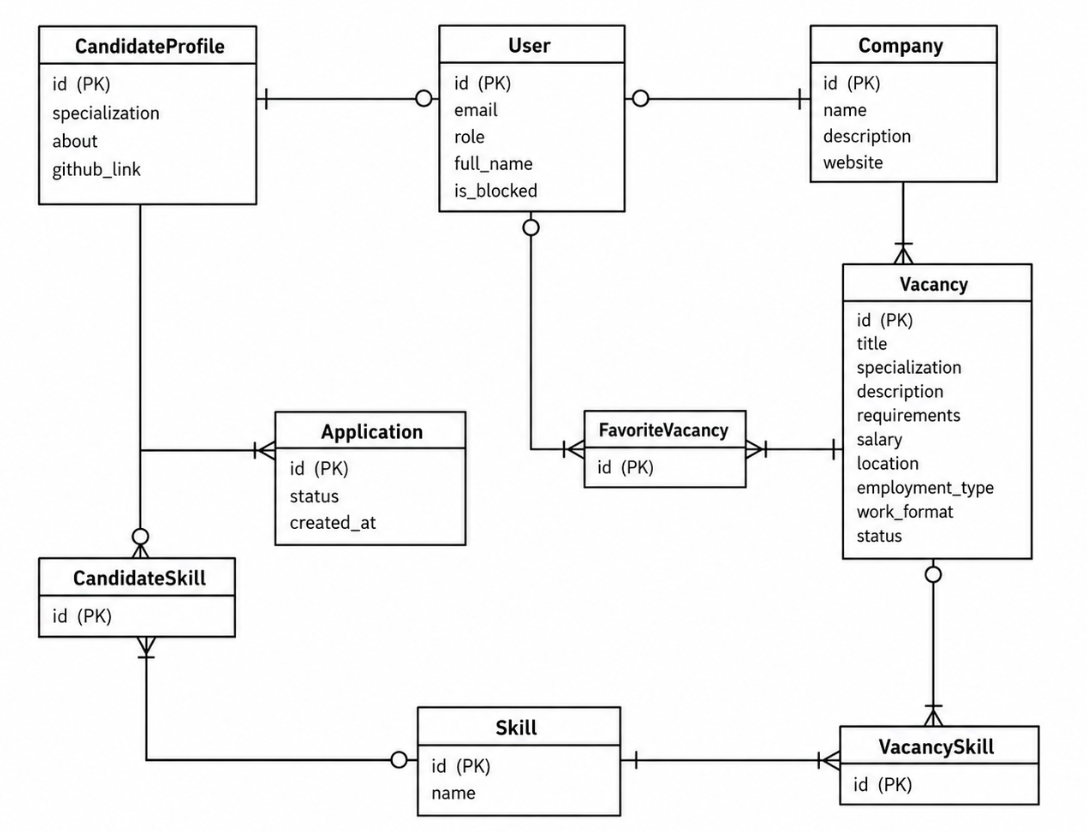
\includegraphics[width=\linewidth]{fig_3_5_er_diagram.png}
	\caption{ER-диаграмма базы данных}
	\label{fig:er_diagram}
\end{figure}

\subsubsection{Нормализация}

Структура базы данных разработанной платформы построена таким образом, чтобы минимизировать дублирование данных и разделить сведения по самостоятельным сущностям в соответствии с их назначением. Выделение отдельных таблиц для пользователей, профилей соискателей, компаний, вакансий, навыков, откликов и избранных вакансий позволяет хранить данные раздельно и связывать их между собой через первичные и внешние ключи. Такое проектное решение соответствует принципам нормализации и обеспечивает логически согласованную организацию данных.

Первая нормальная форма обеспечивается тем, что каждая таблица имеет первичный ключ, а значения атрибутов хранятся в отдельных полях записей. В модели отсутствуют повторяющиеся группы атрибутов внутри одной таблицы: сведения о пользователе хранятся в таблице User, профессиональные данные соискателя — в CandidateProfile, сведения о работодателе — в Company, а информация о вакансии — в Vacancy. Благодаря этому данные предметной области не объединяются в одну крупную запись, а распределяются по специализированным сущностям.

Признаки второй нормальной формы проявляются в том, что данные, относящиеся к разным объектам предметной области, вынесены в отдельные таблицы и не зависят от части составного отношения. Это особенно заметно в таблицах, реализующих связи между сущностями. Например, связь между профилем соискателя и навыком оформлена через таблицу CandidateSkill, а связь между вакансией и навыком — через таблицу VacancySkill. Аналогично добавление вакансии в избранное вынесено в таблицу FavoriteVacancy, а факт отклика на вакансию — в таблицу Application. Благодаря такому разбиению информация о навыках, откликах и избранных вакансиях не дублируется в основных таблицах и хранится в виде самостоятельных связующих сущностей.

Третья нормальная форма обеспечивается тем, что сведения, логически относящиеся к отдельным объектам, не переносятся в зависимые таблицы. Так, данные компании хранятся в таблице Company и связываются с вакансиями через внешний ключ companyId, поэтому сведения о работодателе не дублируются в каждой записи Vacancy. Аналогично сведения о пользователе хранятся в таблице User, тогда как профессиональные характеристики соискателя вынесены в CandidateProfile и связаны с учётной записью через userId. Это устраняет транзитивное дублирование и позволяет изменять данные пользователя, профиля или компании независимо друг от друга.

Дополнительным примером нормализованной структуры является использование таблицы Skill как общего справочника навыков. Вместо хранения текстовых названий навыков непосредственно в профилях соискателей и вакансиях используется единая сущность Skill, связанная с ними через отдельные ассоциативные таблицы. Это позволяет исключить повторение одинаковых значений навыков в разных частях базы данных и упростить поддержку единого перечня компетенций.

Таким образом, структура базы данных платформы соответствует требованиям нормализации на уровне, достаточном для рассматриваемой предметной области. Разделение данных по самостоятельным сущностям, использование внешних ключей и вынесение связей «многие ко многим» в отдельные таблицы позволяют уменьшить избыточность, упростить сопровождение схемы и снизить вероятность аномалий при добавлении, обновлении и удалении данных.

\subsubsection{Реляционная модель данных}

На основе ER-модели, представленной в подразделе 3.5.1, построена реляционная модель базы данных, в которой сущности предметной области представлены в виде таблиц, а связи между ними реализованы посредством первичных и внешних ключей. Реляционная модель определяет состав таблиц, их атрибуты и ограничения целостности, используемые в схеме базы данных платформы. В состав модели входят таблицы users, candidate\_profiles, companies, vacancies, skills, candidate\_skills, vacancy\_skills, applications и favorite\_vacancies.

Для идентификации записей в основных таблицах используются суррогатные первичные ключи id типа BIGINT с автоинкрементом. Такой подход обеспечивает однозначную идентификацию каждой записи и упрощает построение внешних связей между таблицами. Аналогичное решение применяется в таблицах users, vacancies и applications, а также в остальных сущностях схемы базы данных.

Связь между таблицами users и candidate\_profiles реализуется через внешний ключ user\_id, для которого установлено ограничение уникальности. Это означает, что одной учётной записи может соответствовать не более одного профиля соискателя. Аналогичным образом таблица companies связана с users через внешний ключ user\_id с ограничением уникальности, что задаёт отношение «один пользователь — не более одной компании». Таблица vacancies связана с companies через внешний ключ company\_id, благодаря чему одной компании может принадлежать множество вакансий.

Таблица applications связывает вакансии и профили соискателей через внешние ключи vacancy\_id и profile\_id. Для комбинации этих полей установлено ограничение уникальности, исключающее повторную подачу отклика одним и тем же соискателем на одну и ту же вакансию. По аналогичному принципу таблицы candidate\_skills и vacancy\_skills реализуют связи «многие ко многим» между профилями соискателей и навыками, а также между вакансиями и навыками. В таблице favorite\_vacancies связь между пользователем и вакансией также оформлена через пару внешних ключей user\_id и vacancy\_id с ограничением уникальности.

На уровне схемы базы данных определены ограничения целостности, соответствующие логике предметной области. В таблице users поле email имеет ограничение уникальности, исключающее регистрацию нескольких пользователей с одним и тем же адресом электронной почты. Для обязательных атрибутов основных сущностей используются ограничения NOT NULL, например для полей email, password\_hash, role в таблице users, а также для title, specialization, description, requirements, employment\_type, work\_format и status в таблице vacancies.

Допустимые значения ряда атрибутов контролируются не только на уровне приложения, но и на уровне схемы базы данных. В частности, для поля role таблицы users, а также для статусных и классификационных полей таблиц vacancies и applications заданы CHECK-ограничения, фиксирующие допустимые значения ролей, статусов вакансий и откликов, типов занятости и форматов работы. Это повышает надёжность хранения данных и снижает риск записи значений, не соответствующих предметной области системы.

Таким образом, реляционная модель базы данных платформы представляет собой набор взаимосвязанных таблиц, отражающих пользователей, профили соискателей, компании, вакансии, навыки, отклики и избранные вакансии. Использование первичных и внешних ключей, ограничений уникальности, NOT NULL и CHECK обеспечивает целостность данных и соответствует требованиям, предъявляемым к хранению информации в разработанной системе.

\subsubsection{Описание структуры таблиц}

Реляционная модель базы данных реализована в виде набора взаимосвязанных таблиц, соответствующих основным сущностям предметной области. В данном подразделе приводится краткое описание назначения таблиц и их роли в логике работы программной системы. Детальная структура каждой таблицы представлена непосредственно в соответствующей таблице.

Таблица \texttt{users} используется как базовая таблица учётных записей программной системы. Она обеспечивает хранение данных пользователей и служит основой для разграничения доступа между соискателем, работодателем и администратором. Структура таблицы \texttt{users} приведена в таблице~\ref{tab:users}.

\begingroup
\renewcommand{\baselinestretch}{1}\selectfont
\renewcommand{\arraystretch}{1.2}
\setlength{\extrarowheight}{3pt}

\begin{xltabular}{\textwidth}{|C{2.3cm}|C{2.8cm}|>{\raggedright\arraybackslash}m{4.8cm}|C{2.8cm}|C{1.4cm}|}
	\caption{Атрибуты таблицы \texttt{users} (Пользователи)}\label{tab:users}\\ \hline
	Key Type & Optionality & \multicolumn{1}{c|}{Column name} & Data Type & Size \\ \hline
	PK & * & id & BIGINT & \\ \hline
	UK & * & email & VARCHAR & 255 \\ \hline
	& * & password\_hash & VARCHAR & 255 \\ \hline
	& * & role & VARCHAR & 20 \\ \hline
	& * & full\_name & VARCHAR & 255 \\ \hline
	&   & is\_blocked & BOOLEAN & \\ \hline
\end{xltabular}

\endgroup

Таблица \texttt{candidate\_profiles} предназначена для хранения профессионального профиля соискателя. В рамках разработанной системы этот профиль выполняет роль резюме, поэтому отдельная сущность резюме не создаётся. Таблица используется при просмотре и фильтрации кандидатов работодателем. Структура таблицы \texttt{candidate\_profiles} приведена в таблице~\ref{tab:candidate_profiles}.

\begingroup
\renewcommand{\baselinestretch}{1}\selectfont
\renewcommand{\arraystretch}{1.2}
\setlength{\extrarowheight}{3pt}

\begin{xltabular}{\textwidth}{|C{2.3cm}|C{2.8cm}|>{\raggedright\arraybackslash}m{4.8cm}|C{2.8cm}|C{1.4cm}|}
	\caption{Атрибуты таблицы \texttt{candidate\_profiles} (Профили соискателей)}\label{tab:candidate_profiles}\\ \hline
	Key Type & Optionality & \multicolumn{1}{c|}{Column name} & Data Type & Size \\ \hline
	PK & * & id & BIGINT & \\ \hline
	FK, UK & * & user\_id & BIGINT & \\ \hline
	& * & specialization & VARCHAR & 100 \\ \hline
	&   & about & TEXT & \\ \hline
	&   & github\_link & VARCHAR & 255 \\ \hline
\end{xltabular}

\endgroup

Таблица \texttt{companies} используется для хранения сведений об организациях-работодателях. Она связывает работодателя с компанией, от имени которой создаются и публикуются вакансии. Структура таблицы \texttt{companies} приведена в таблице~\ref{tab:companies}.

\begingroup
\renewcommand{\baselinestretch}{1}\selectfont
\renewcommand{\arraystretch}{1.2}
\setlength{\extrarowheight}{3pt}

\begin{xltabular}{\textwidth}{|C{2.3cm}|C{2.8cm}|>{\raggedright\arraybackslash}m{4.8cm}|C{2.8cm}|C{1.4cm}|}
	\caption{Атрибуты таблицы \texttt{companies} (Компании)}\label{tab:companies}\\ \hline
	Key Type & Optionality & \multicolumn{1}{c|}{Column name} & Data Type & Size \\ \hline
	PK & * & id & BIGINT & \\ \hline
	FK, UK & * & user\_id & BIGINT & \\ \hline
	& * & name & VARCHAR & 255 \\ \hline
	&   & description & TEXT & \\ \hline
	&   & website & VARCHAR & 255 \\ \hline
\end{xltabular}

\endgroup

Таблица \texttt{vacancies} предназначена для хранения вакансий, создаваемых работодателями. Она отражает основную сущность, через которую соискатель получает информацию о предложении работы, а работодатель управляет публикацией и дальнейшей обработкой откликов. Структура таблицы \texttt{vacancies} приведена в таблице~\ref{tab:vacancies}.

\begingroup
\renewcommand{\baselinestretch}{1}\selectfont
\renewcommand{\arraystretch}{1.2}
\setlength{\extrarowheight}{3pt}

\begin{xltabular}{\textwidth}{|C{2.3cm}|C{2.8cm}|>{\raggedright\arraybackslash}m{4.8cm}|C{2.8cm}|C{1.4cm}|}
	\caption{Атрибуты таблицы \texttt{vacancies} (Вакансии)}\label{tab:vacancies}\\ \hline
	Key Type & Optionality & \multicolumn{1}{c|}{Column name} & Data Type & Size \\ \hline
	PK & * & id & BIGINT & \\ \hline
	FK & * & company\_id & BIGINT & \\ \hline
	& * & title & VARCHAR & 255 \\ \hline
	& * & specialization & VARCHAR & 100 \\ \hline
	& * & description & TEXT & \\ \hline
	& * & requirements & TEXT & \\ \hline
	&   & salary & VARCHAR & 100 \\ \hline
	&   & location & VARCHAR & 255 \\ \hline
	& * & employment\_type & VARCHAR & \\ \hline
	& * & work\_format & VARCHAR & \\ \hline
	& * & status & VARCHAR & \\ \hline
	&   & created\_at & DATE & \\ \hline
\end{xltabular}

\endgroup

Таблица \texttt{skills} представляет единый справочник навыков, используемых в системе. Наличие отдельного справочника позволяет применять один и тот же перечень компетенций как для описания профилей соискателей, так и для указания требований вакансий. Структура таблицы \texttt{skills} приведена в таблице~\ref{tab:skills}.

\newpage
\begingroup
\renewcommand{\baselinestretch}{1}\selectfont
\renewcommand{\arraystretch}{1.2}
\setlength{\extrarowheight}{3pt}

\begin{xltabular}{\textwidth}{|C{2.3cm}|C{2.8cm}|>{\raggedright\arraybackslash}m{4.8cm}|C{2.8cm}|C{1.4cm}|}
	\caption{Атрибуты таблицы \texttt{skills} (Навыки)}\label{tab:skills}\\ \hline
	Key Type & Optionality & \multicolumn{1}{c|}{Column name} & Data Type & Size \\ \hline
	PK & * & id & BIGINT & \\ \hline
	UK & * & name & VARCHAR & 100 \\ \hline
\end{xltabular}

\endgroup

Таблица \texttt{candidate\_skills} используется для связи профилей соискателей с навыками. Она позволяет одному профилю иметь несколько навыков и одновременно использовать один и тот же навык в разных профилях. Структура таблицы \texttt{candidate\_skills} приведена в таблице~\ref{tab:candidate_skills}.

\begingroup
\renewcommand{\baselinestretch}{1}\selectfont
\renewcommand{\arraystretch}{1.2}
\setlength{\extrarowheight}{3pt}

\begin{xltabular}{\textwidth}{|C{2.3cm}|C{2.8cm}|>{\raggedright\arraybackslash}m{4.8cm}|C{2.8cm}|C{1.4cm}|}
	\caption{Атрибуты таблицы \texttt{candidate\_skills} (Навыки соискателей)}\label{tab:candidate_skills}\\ \hline
	Key Type & Optionality & \multicolumn{1}{c|}{Column name} & Data Type & Size \\ \hline
	PK & * & id & BIGINT & \\ \hline
	FK & * & profile\_id & BIGINT & \\ \hline
	FK & * & skill\_id & BIGINT & \\ \hline
\end{xltabular}

\endgroup

Таблица \texttt{vacancy\_skills} используется для связи вакансий с навыками. Она позволяет работодателю указывать несколько требуемых компетенций для одной вакансии и переиспользовать общий справочник навыков в разных вакансиях. Структура таблицы \texttt{vacancy\_skills} приведена в таблице~\ref{tab:vacancy_skills}.

\begingroup
\renewcommand{\baselinestretch}{1}\selectfont
\renewcommand{\arraystretch}{1.2}
\setlength{\extrarowheight}{3pt}

\begin{xltabular}{\textwidth}{|C{2.3cm}|C{2.8cm}|>{\raggedright\arraybackslash}m{4.8cm}|C{2.8cm}|C{1.4cm}|}
	\caption{Атрибуты таблицы \texttt{vacancy\_skills} (Навыки вакансий)}\label{tab:vacancy_skills}\\ \hline
	Key Type & Optionality & \multicolumn{1}{c|}{Column name} & Data Type & Size \\ \hline
	PK & * & id & BIGINT & \\ \hline
	FK & * & vacancy\_id & BIGINT & \\ \hline
	FK & * & skill\_id & BIGINT & \\ \hline
\end{xltabular}

\endgroup

Таблица \texttt{applications} фиксирует факт отклика соискателя на конкретную вакансию. Она используется для организации процесса рассмотрения кандидата работодателем и отслеживания состояния отклика в рамках пользовательского сценария подбора. Структура таблицы \texttt{applications} приведена в таблице~\ref{tab:applications}.

\begingroup
\renewcommand{\baselinestretch}{1}\selectfont
\renewcommand{\arraystretch}{1.2}
\setlength{\extrarowheight}{3pt}

\begin{xltabular}{\textwidth}{|C{2.3cm}|C{2.8cm}|>{\raggedright\arraybackslash}m{4.8cm}|C{2.8cm}|C{1.4cm}|}
	\caption{Атрибуты таблицы \texttt{applications} (Отклики)}\label{tab:applications}\\ \hline
	Key Type & Optionality & \multicolumn{1}{c|}{Column name} & Data Type & Size \\ \hline
	PK & * & id & BIGINT & \\ \hline
	FK & * & vacancy\_id & BIGINT & \\ \hline
	FK & * & profile\_id & BIGINT & \\ \hline
	& * & status & VARCHAR & 20 \\ \hline
	&   & created\_at & DATE & \\ \hline
\end{xltabular}

\endgroup

Таблица \texttt{favorite\_vacancies} предназначена для хранения вакансий, добавленных пользователями в избранное. Она поддерживает сценарий сохранения интересующих предложений для последующего просмотра без дублирования данных о самих вакансиях. Структура таблицы \texttt{favorite\_vacancies} приведена в таблице~\ref{tab:favorite_vacancies}.

\begingroup
\renewcommand{\baselinestretch}{1}\selectfont
\renewcommand{\arraystretch}{1.2}
\setlength{\extrarowheight}{3pt}

\begin{xltabular}{\textwidth}{|C{2.3cm}|C{2.8cm}|>{\raggedright\arraybackslash}m{4.8cm}|C{2.8cm}|C{1.4cm}|}
	\caption{Атрибуты таблицы \texttt{favorite\_vacancies} (Избранные вакансии)}\label{tab:favorite_vacancies}\\ \hline
	Key Type & Optionality & \multicolumn{1}{c|}{Column name} & Data Type & Size \\ \hline
	PK & * & id & BIGINT & \\ \hline
	FK & * & user\_id & BIGINT & \\ \hline
	FK & * & vacancy\_id & BIGINT & \\ \hline
\end{xltabular}

\endgroup

Таким образом, описание структуры таблиц базы данных отражает назначение основных сущностей программной системы и их участие в пользовательских сценариях: регистрации, ведении профилей, публикации вакансий, работе с навыками, отправке откликов и сохранении избранных вакансий. Подробные сведения о составе таблиц приведены непосредственно в таблицах 3.1--3.9.

\subsection{Эксплуатация и развёртывание}

Для развёртывания платформы и обеспечения единообразия программного окружения используется контейнеризация на основе Docker. Такой подход позволяет изолировать основные компоненты системы, упростить запуск приложения и базы данных, а также снизить влияние различий в конфигурации хост-машины при разработке, тестировании и демонстрации проекта. Конфигурация окружения задана в файле docker-compose.yml и предусматривает запуск двух основных сервисов: приложения и базы данных.

Сервис app представляет собой контейнер серверного приложения. Его сборка выполняется на основе локального Dockerfile, в котором в качестве базового образа используется node:22-alpine. В процессе сборки рабочая директория устанавливается в каталог /app, затем копируются файлы зависимостей, выполняется установка пакетов командой npm ci, после чего в контейнер переносится исходный код проекта. В качестве команды запуска используется npm start, а приложение экспонируется на порту 3000.

Сервис db представляет собой контейнер базы данных и использует официальный образ postgres:16-alpine. Для инициализации экземпляра PostgreSQL в конфигурации заданы переменные окружения POSTGRES\_USER, POSTGRES\_PASSWORD и POSTGRES\_DB. Данные базы сохраняются во внешнем томе postgres\_data, что позволяет сохранять состояние БД при перезапуске контейнеров. Для контроля готовности сервиса базы данных используется healthcheck, выполняющий проверку доступности PostgreSQL командой pg\_isready.

Контейнер приложения получает параметры подключения к базе данных через переменные окружения DB\_HOST, DB\_PORT, DB\_USER, DB\_PASSWORD, DB\_NAME и DB\_DIALECT. Внутри конфигурации в качестве хоста базы данных используется имя сервиса db, что обеспечивает взаимодействие между контейнерами в пределах сети Docker Compose. Для запуска приложения только после готовности базы данных в конфигурации сервиса app используется директива depends\_on с условием service\_healthy.

Инициализация схемы базы данных в проекте выполняется не через автоматическое создание таблиц по моделям, а с помощью миграций Sequelize CLI. В составе проекта предусмотрены команды npm run db:migrate, npm run db:seed и npm run db:reset, позволяющие развернуть схему, заполнить справочные данные и при необходимости полностью пересоздать структуру базы данных. Такой подход обеспечивает воспроизводимое создание схемы и согласованность структуры БД с кодом проекта.

Таким образом, выбранный способ развёртывания обеспечивает воспроизводимость программного окружения, изоляцию серверного приложения и базы данных, а также упрощает запуск системы в рамках разработки и демонстрации. Использование Docker Compose, отдельных контейнеров app и db, механизма проверки готовности базы данных и миграций Sequelize CLI соответствует архитектуре разработанной платформы и упрощает её сопровождение.

